\chapter{Normal (Gaussian) Distribution/ Gauss curve ($X \sim \mathcal{N}(\mu,\sigma^2)$/ $\mathcal{N}(\mu, \Sigma)$) \cite{ism-1,mfml-1,wiki/Normal_distribution}} \label{Normal (Gaussian) Distribution}

\begin{table}[H]
    \begin{minipage}{0.49\linewidth}
        \begin{figure}[H]
            \centering
            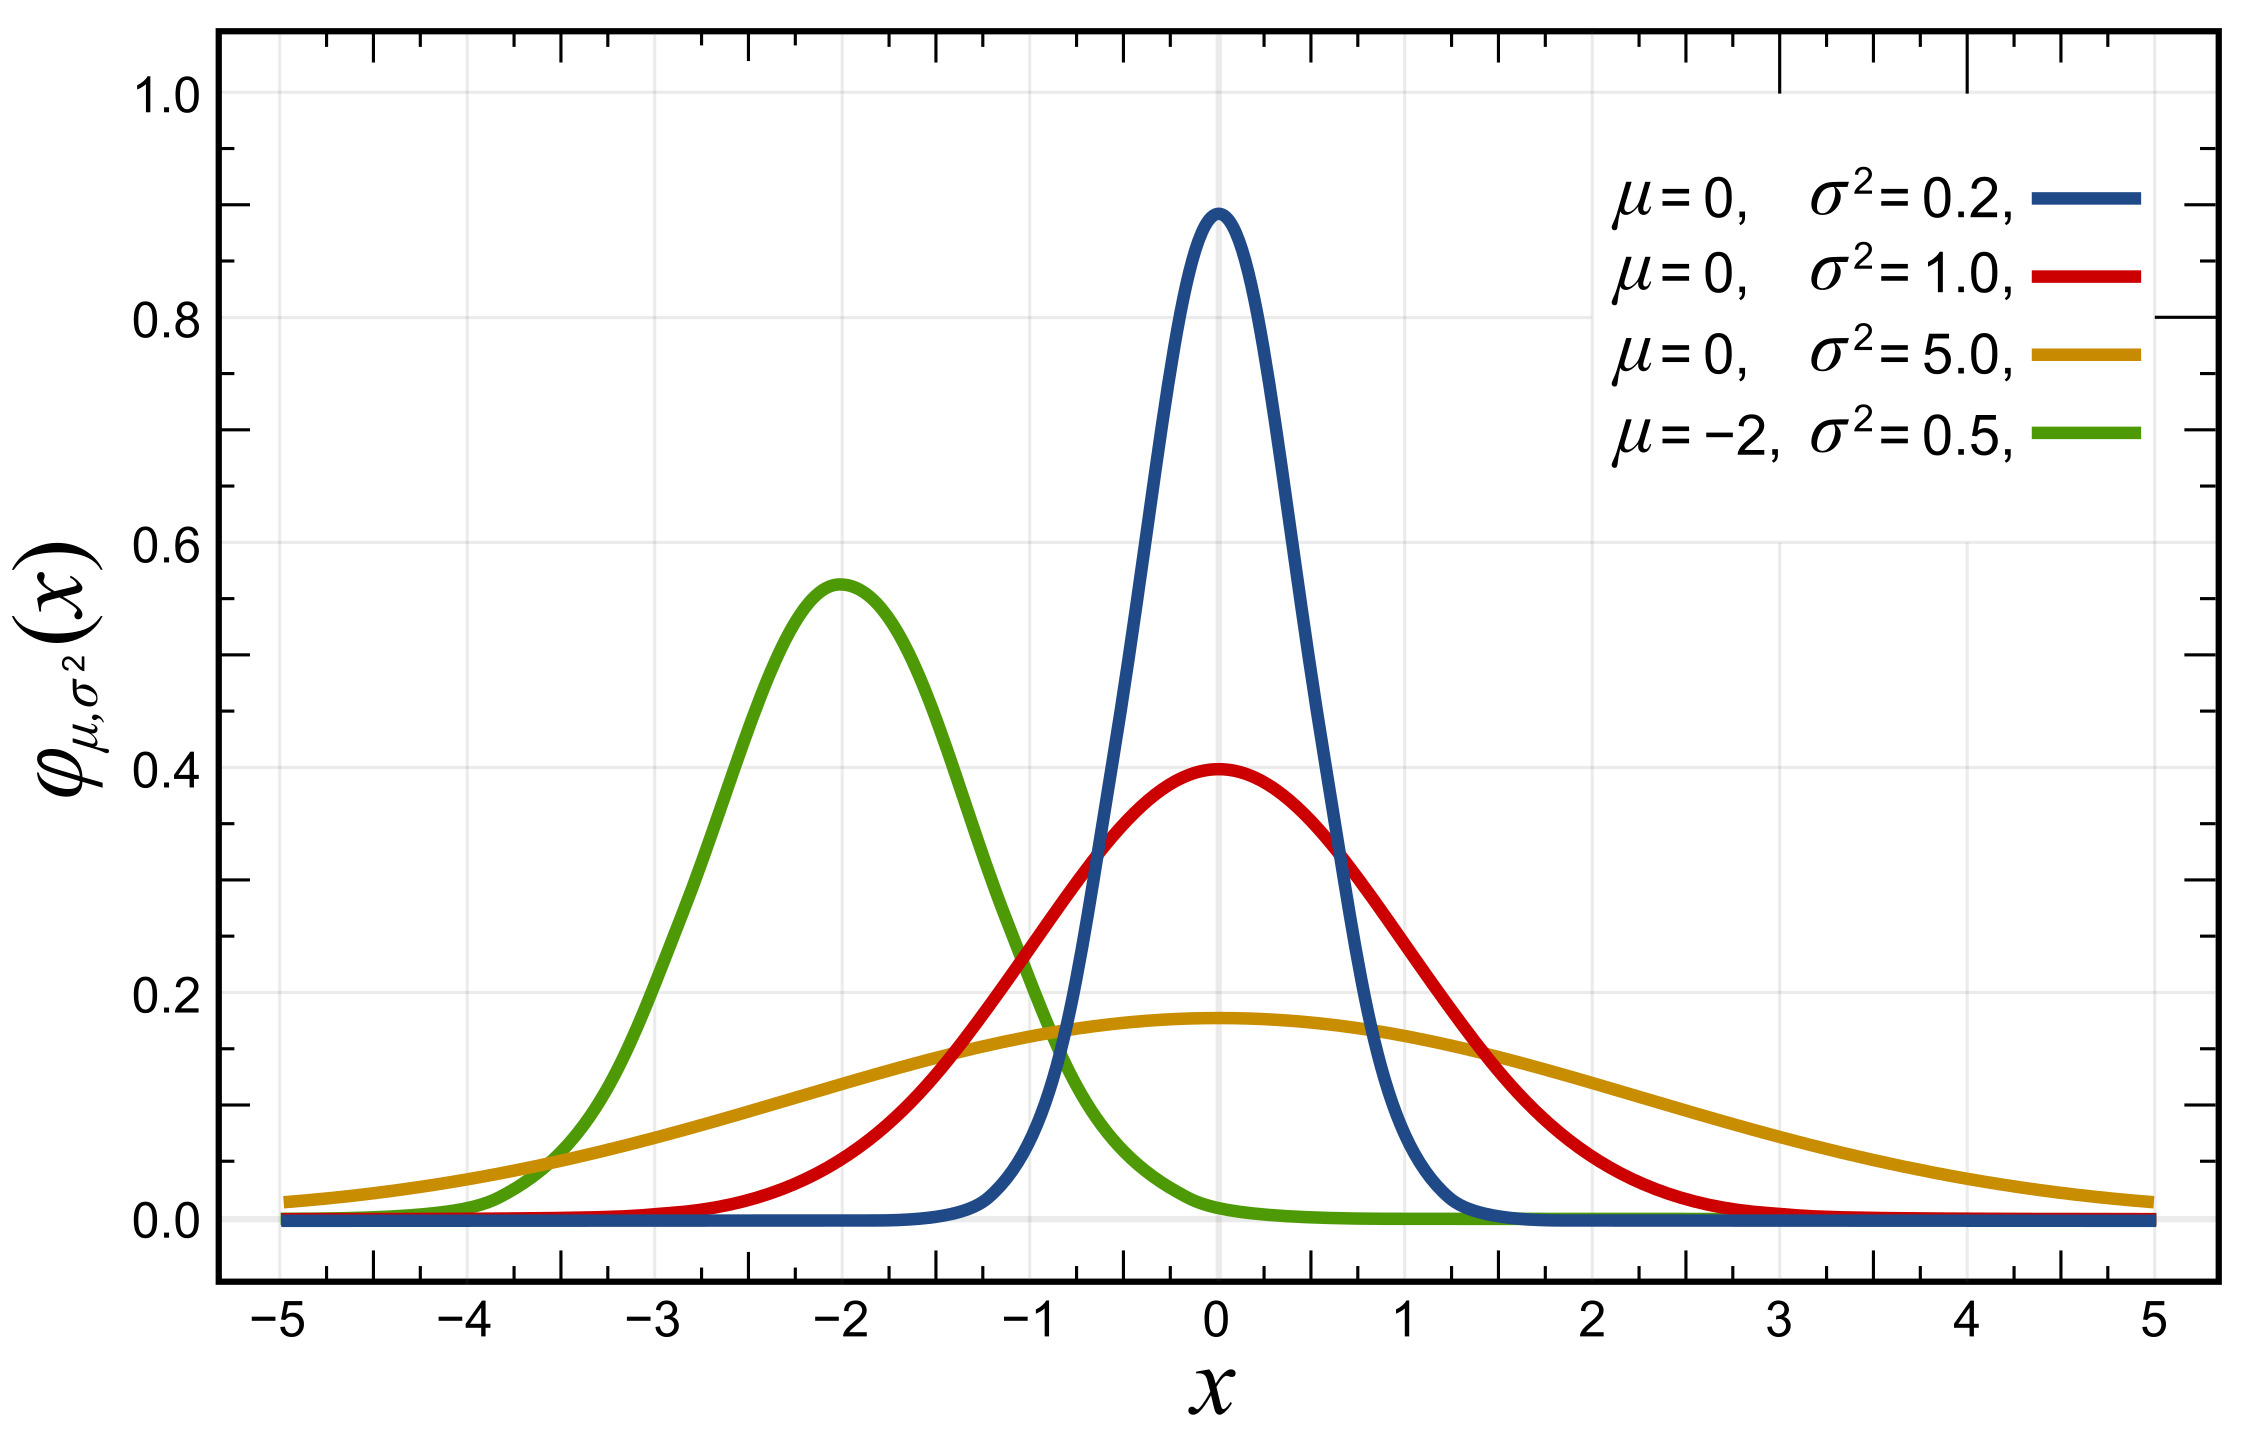
\includegraphics[width=\linewidth, height=4cm, keepaspectratio]{Pictures/distributions/Normal_Distribution_PDF.jpg}
            \caption{Normal distribution: PDF}
        \end{figure}
    \end{minipage}
    \hfill
    \begin{minipage}{0.49\linewidth}
        \begin{figure}[H]
            \centering
            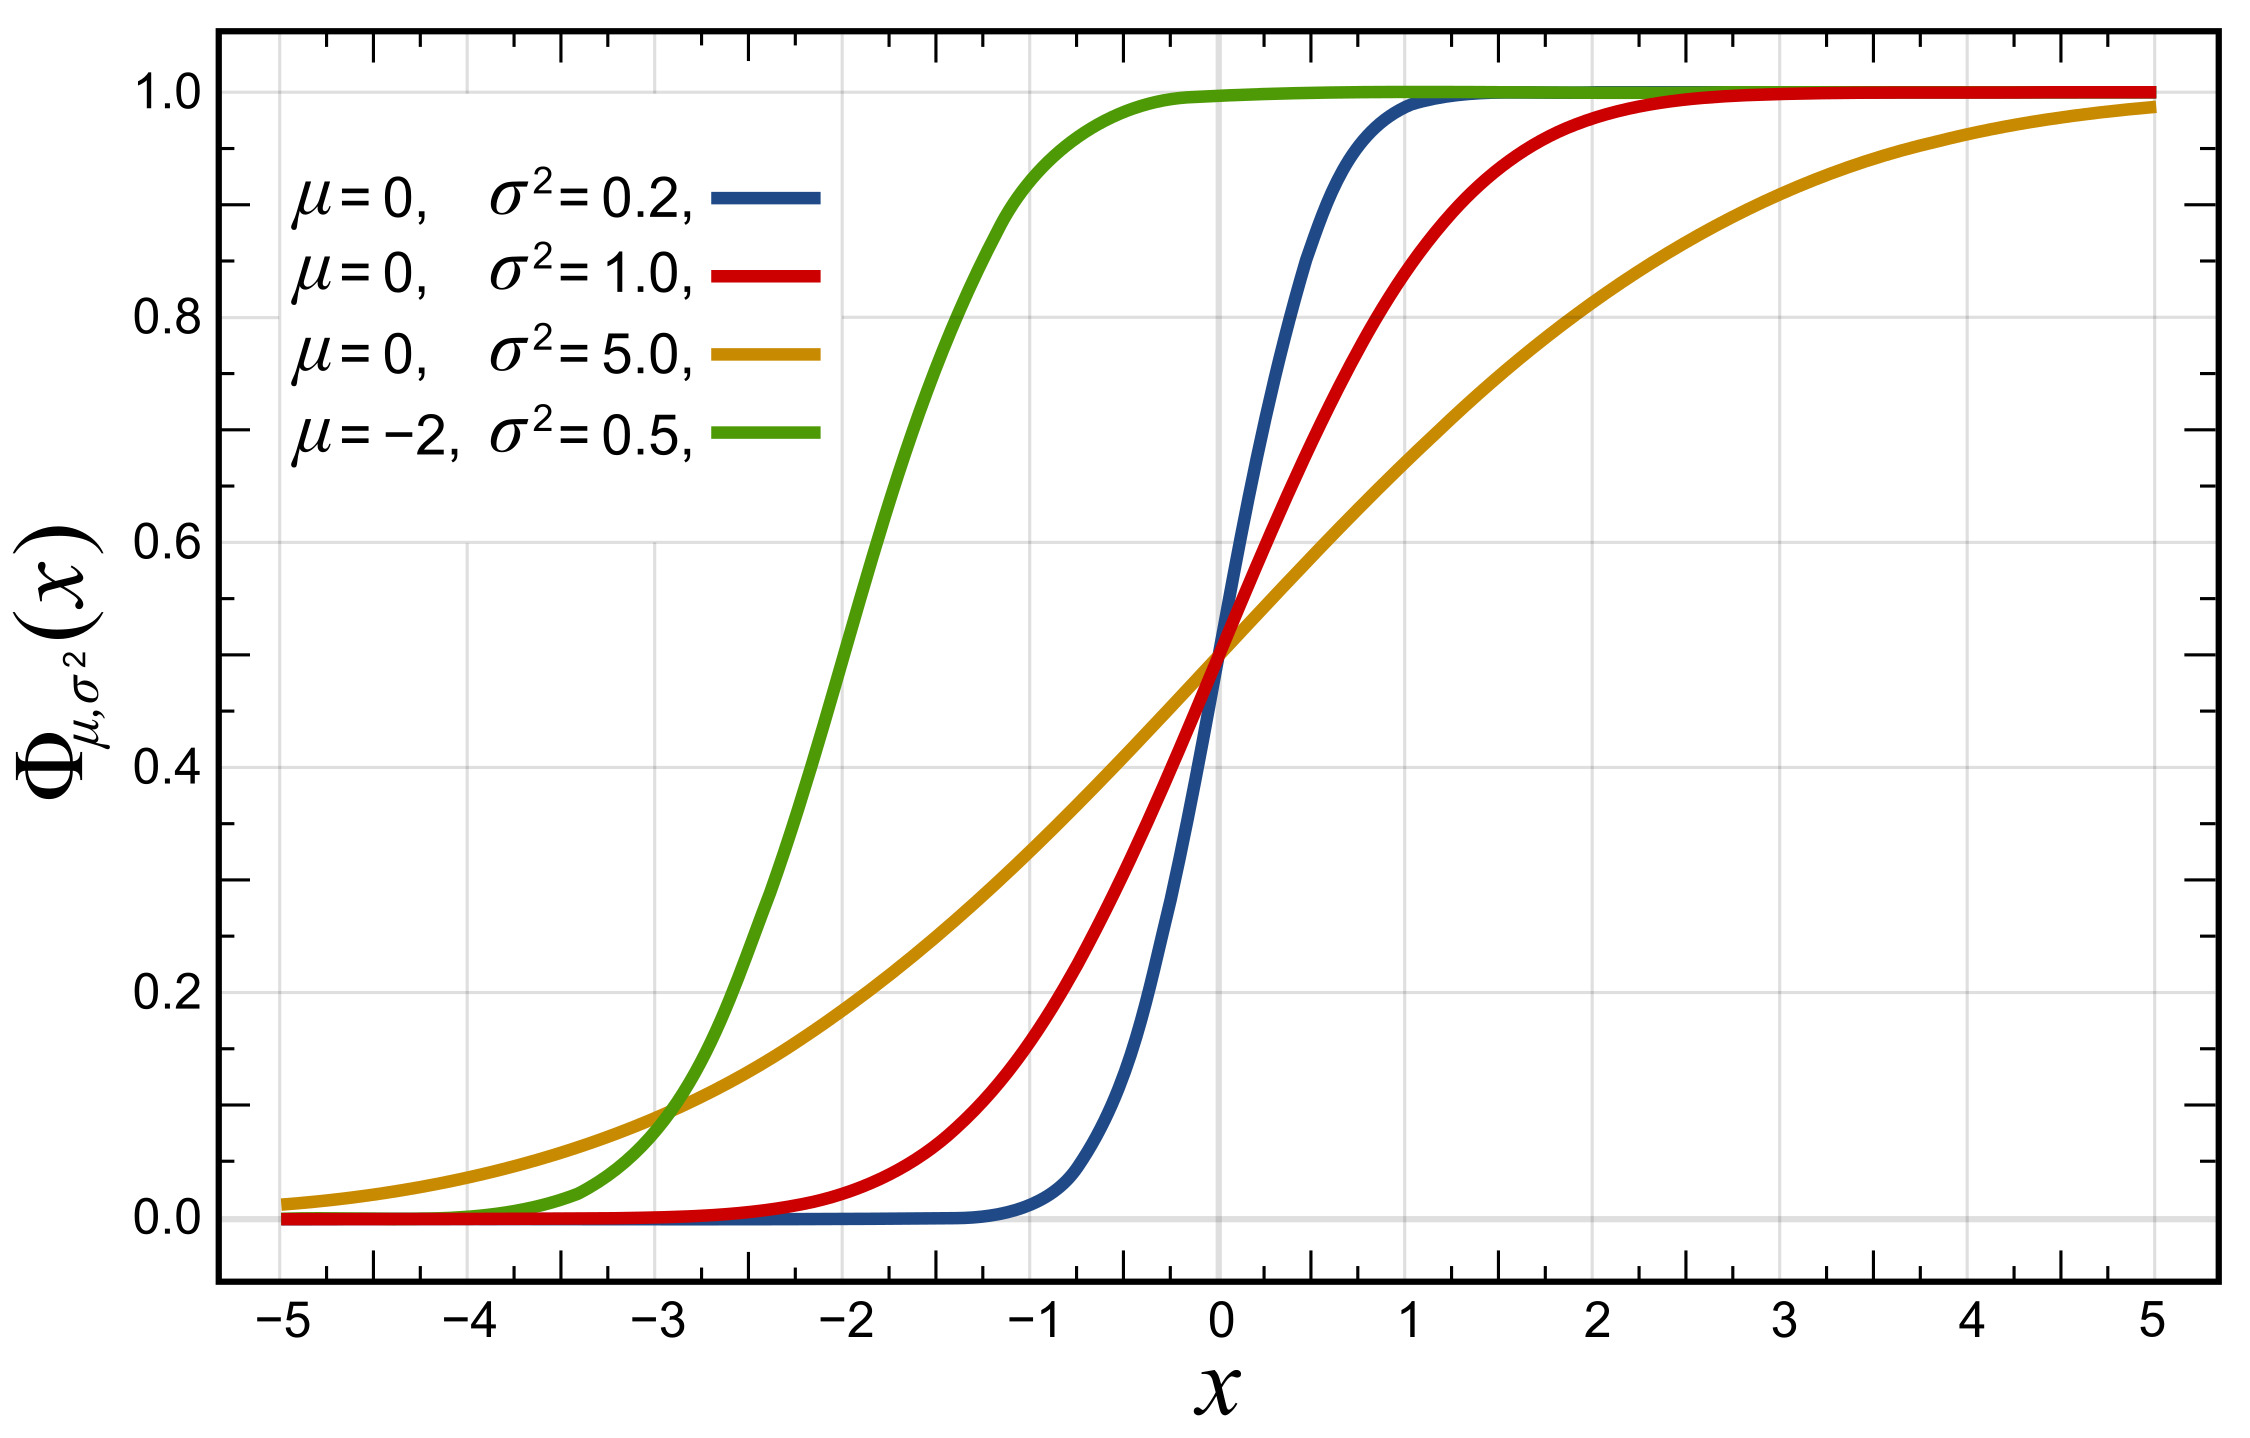
\includegraphics[width=\linewidth, height=4cm, keepaspectratio]{Pictures/distributions/Normal_Distribution_CDF.jpg}
            \caption{Normal distribution: CDF}
        \end{figure}
    \end{minipage}
\end{table}

\renewcommand{\arraystretch}{2}
\begin{longtable}{|m{6cm}|p{9cm}|}
    \hline
    \multicolumn{2}{|c|}{\textbf{Normal (Gaussian) Distribution/ Gauss curve - Info} \cite{wiki/Normal_distribution}} \\
    \hline\endfirsthead

    \hline
    \multicolumn{2}{|c|}{\textbf{Normal (Gaussian) Distribution/ Gauss curve - Info - contd.} \cite{wiki/Normal_distribution}} \\
    \hline\endhead
    
    \hline\endfoot
    \hline\endlastfoot

    \hline
    \textbf{Notation} & 
    ${\displaystyle {\mathcal {N}}(\mu ,\sigma ^{2})}$ 
    \\ \hline

    \textbf{Statistical parameters} & 
    \tableenumerate{
        \item ${\displaystyle \mu \in \mathbb {R} }$ = mean (location)
        
        \item ${\displaystyle \sigma ^{2}\in \mathbb {R} _{>0}}$ = variance (squared scale)
    }
    \\ \hline
    
    \textbf{Support} & 
    ${\displaystyle x\in \mathbb {R} }$
    \\ \hline

    \textbf{Probability Density Function (PDF)} & 
    $\vspace{0.1cm}{\displaystyle {\dfrac {1}{\sqrt {2\pi \sigma ^{2}}}}e^{-{\dfrac {(x-\mu )^{2}}{2\sigma ^{2}}}}}$
    \\[2ex] \hline
    
    \textbf{Cumulative distribution function (CDF)} & 
    ${\displaystyle \Phi \left({\dfrac {x-\mu }{\sigma }}\right)={\dfrac {1}{2}}\left[1+\operatorname {erf} \left({\dfrac {x-\mu }{\sigma {\sqrt {2}}}}\right)\right]}$
    \\ \hline

    \textbf{Quantile} &
    ${\displaystyle \mu +\sigma {\sqrt {2}}\operatorname {erf} ^{-1}(2p-1)}$
    \\ \hline

    \textbf{Mean} & 
    $\mu$
    \\ \hline

    \textbf{Median} & 
    $\mu$
    \\ \hline

    \textbf{Mode} & 
    $\mu$
    \\ \hline

    \textbf{Variance} &
    $\sigma^2$
    \\ \hline

    \textbf{Mean absolute deviation (MAD)} &
    ${\displaystyle \sigma {\sqrt {\dfrac{2}{\pi} }}}$ 
    \\[1ex] \hline

    \textbf{Skewness} &
    $0$ 
    \\ \hline

    \textbf{Excess kurtosis} &
    $0$ 
    \\ \hline

    \textbf{Entropy} &
    ${\displaystyle {\dfrac {1}{2}}\log(2\pi e\sigma ^{2})}$
    \\[1ex] \hline

    \textbf{Moment-generating function (MGF)} &
    ${\displaystyle \exp(\mu t+\dfrac{\sigma ^{2}t^{2}}{2})}$
    \\[1ex] \hline

    \textbf{Characteristic function (CF)} &
    ${\displaystyle \exp(i\mu t-\dfrac{\sigma ^{2}t^{2}}{2})}$
    \\[1ex] \hline

    \textbf{Fisher information} &
    \tableenumerate{
        \item ${\displaystyle {\mathcal {I}}(\mu ,\sigma )={\begin{pmatrix}1/\sigma ^{2}&0\\0&2/\sigma ^{2}\end{pmatrix}}}$
        \vspace{0.1cm}

        \item ${\displaystyle {\mathcal {I}}(\mu ,\sigma ^{2})={\begin{pmatrix}1/\sigma ^{2}&0\\0&1/(2\sigma ^{4})\end{pmatrix}}}$
        \vspace{0.1cm}
    }
    \\[1ex] \hline

    \textbf{Kullback–Leibler divergence} &
    ${\displaystyle {1 \over 2}\left\{\left({\frac {\sigma _{0}}{\sigma _{1}}}\right)^{2}+{\frac {(\mu _{1}-\mu _{0})^{2}}{\sigma _{1}^{2}}}-1+\ln {\sigma _{1}^{2} \over \sigma _{0}^{2}}\right\}}$
    \\[2ex] \hline

\end{longtable}
\renewcommand{\arraystretch}{1}


\begin{enumerate}
    \item First introduced explicitly as a PDF by Carl Friedrich Gauss, and it is therefore often referred to as the \textbf{Gauss curve} \indexlabel{Gauss curve}
\end{enumerate}

\section{Probability Density Function (PDF) ($f_{\mu,\sigma}(x)$ / $p(x|\mu,\sigma^2)$) \cite{ism-1,mfml-1}} \label{Normal Distribution: PDF}

\[
    p(x|\mu,\sigma^2)
    = f_{\mu,\sigma}(x)
    = \dfrac{1}{\sqrt{2\pi\sigma^2}}
    \exp\dParenBrac{
        -\dfrac{(x - \mu)^2}{2\sigma^2}
    }
    = \dfrac{1}{\sigma}\phi\dParenBrac{
        \dfrac{x - \mu}{\sigma}
    }
\]


\section{Cumulative Distribution Function (CDF) ($F_{\mu,\sigma}(x)$/ $\Phi\dParenBrac{ \frac{x-\mu}{\sigma} }$) \cite{ism-1}} \label{Normal Distribution: CDF}

\[
    \Phi\dParenBrac{\dfrac{x-\mu}{\sigma}}
    = F_{\mu,\sigma}(x)
    = Pr(X \leq x)
    = \dint_{-\infty}^x \dfrac{1}{\sigma}\phi\dParenBrac{
        \dfrac{z - \mu}{\sigma}
    } dz
    = \dint_{-\infty}^{(x - \mu)/\sigma} \phi(z) dz
\]
\[
    \Phi(x) = \dint_{-\infty}^{x} \phi(z) dz
\]


\section{Properties \cite{ism-1}}

\begin{enumerate}
    \item $z_p = -z_{1-p}$

    \item The sum of the random variables $\dsum_{i=1}^{n} X_i$ is again normally distributed, but now with mean $n\mu$ and variance $n\sigma^2$
\end{enumerate}

\section{Confidence Interval \cite{ism-1}}


\begin{enumerate}[itemsep=0.5cm]
    \item $\dfrac{\bar{X} - \mu}{\sigma/\sqrt{n}}$ is standard normal distributed

    \item $V_{n-1}^2 = (n-1)S^2/\sigma^2 \sim \chi_{n-1}^2$ is chi-square distributed

    \item $
        \dfrac{\bar{X} - \mu}{S/\sqrt{n}}
        = \dfrac{
            {(\bar{X} - \mu)}/{(\sigma/\sqrt{n})}
        }{
            \sqrt{(n-1)S^2/\sigma^2}/\sqrt{n-1}
        }
        =\dfrac{Z}{V_{n-1}/\sqrt{n-1}}
    $

    \item $\dfrac{\bar{X} - \mu}{S/\sqrt{n}}$ is student t distributed (DOF: $n-1$)

    \item Popular Confidence Intervals:
    \begin{table}[H]
        \centering
        \begin{tabular}{r l l}
            $95\%$ & $[\mu - 1.96\sigma,$ & $\mu + 1.96\sigma]$ \\
            
            $95.45\%$ &  $[\mu - 2\sigma,$ & $\mu + 2\sigma]$ \\

            $99.73\%$ & $[\mu - 3\sigma,$ & $\mu + 3\sigma]$ \\

        \end{tabular}
    \end{table}

\end{enumerate}

\section{Bivariate/ Multivariate \cite{ism-1,mfml-1}} \label{Normal distribution: Bivariate/ Multivariate}

\begin{table}[H]
    \centering
    \begin{tabular}{l l}
        $\rho$ & correlation coefficient\\
        
    \end{tabular}
\end{table}

if $\rho = 0$, $X \& Y$ are \textbf{independent}

\subsection{Probability Density Function (PDF) \cite{ism-1,mfml-1}} \label{Normal distribution: Bivariate/ Multivariate: PDF}

\begin{enumerate}[itemsep=0.5cm]
    \item $
        \hfill
        z_1 = \dfrac{x - \mu_X}{\sigma_X}
        \hfill
        z_2 = \dfrac{y - \mu_Y}{\sigma_Y}
        \hfill
    $ \hfill \cite{ism-1}
    
    \item $
        f(x,y)
        = \dfrac{1}{
            2\pi \sigma_X \sigma_Y \sqrt{1 - \rho^2}
        }
        \exp\left(
            -\dfrac{z_1^2 - 2\rho z_1z_2 + z_2^2}{2(1 - \rho^2)}
        \right)
    $ \hfill \cite{ism-1}

    \item $
        p(x|\mu, \Sigma)
        = (2\pi)^{-D/2} |\Sigma|^{-1/2}
        \exp(
            -0.5(x - \mu)^\top\Sigma^{-1}(x - \mu)
        )
        \hfill
        (x \in \mathbb{R}^D)
    $ \hfill \cite{mfml-1}

    \item marginal covariance matrix of $x$: $
        \Sigma_{xx} = Co\mathbb{V}[x,x]
    $

    \item marginal covariance matrix of $y$: $
        \Sigma_{yy} = Co\mathbb{V}[y,y]
    $

    \item cross-covariance matrix between x and y: $
        \Sigma_{xy} = \Sigma_{yx} = Co\mathbb{V}[x,y] = Co\mathbb{V}[y,x]
    $

    \item $
        p(x,y)
        = \mathcal{N}\left(
            \begin{bmatrix}
                \mu_x \\ \mu_y
            \end{bmatrix},
            \begin{bmatrix}
                \Sigma_{xx} & \Sigma_{xy} \\ 
                \Sigma_{yx} & \Sigma_{yy} \\ 
            \end{bmatrix}
        \right)
    $ \hfill \cite{mfml-1}
\end{enumerate}

\subsection{conditional distribution \cite{mfml-1}} \label{Normal distribution: Bivariate/ Multivariate: conditional distribution}

\begin{enumerate}[itemsep=0.3cm]
    \item $
        \mu_{x|y} 
        = \mu_x + \Sigma_{xy} \Sigma_{yy}^{-1} (y-\mu_y)
    $

    \item $
        \Sigma_{x|y}
        = \Sigma_{xx} - \Sigma_{xy} \Sigma_{yy}^{-1} \Sigma_{yx}
    $
    
    \item $
        p(x|y) = \mathcal{N}(\mu_{x|y}, \Sigma_{x|y})
    $

    \item in the computation of the mean, the $y$-value is an observation and no longer random
\end{enumerate}


\subsection{marginal distribution \cite{mfml-1}} \label{Normal distribution: Bivariate/ Multivariate: marginal distribution}

\begin{enumerate}[itemsep=0.3cm]
    \item $
        p(x)
        = \dint p(x,y)dy
        = \mathcal{N}(x|\mu_x, \Sigma_{xx})
    $

\end{enumerate}


\subsection{PDF of standardized random variables \cite{ism-1}} \label{Normal distribution: Bivariate/ Multivariate: PDF of standardized random variables}

\[
    \dfrac{
        \exp\{ 
            -(z_1^2 - 2\rho z_1 z_2 + z_2^2)/
            (2(1-\rho^2))
        \}
    }{
        \sqrt{2\pi(1-\rho^2)}
    }
\]


\subsection{Covariance ($COV(X,Y)$) \cite{ism-1}} \label{Normal distribution: Bivariate/ Multivariate: Covariance}

\begin{align*}
    COV(X,Y)
    &= \mathbb{E}(X - \mu_X)(Y - \mu_Y) \\
    &= \sigma_X \sigma_Y \mathbb{E}[Z_1Z_2] \\
    &= \sigma_X \sigma_Y \dint_{-\infty}^{\infty}
        \dint_{-\infty}^{\infty} 
        \dfrac{z_1 z_2}{2\pi (1 - \rho^2)}
        \exp\left\{ 
            -\dfrac{z_1^2 - 2\rho z_1 z_2 + z_2^2}{2(1-\rho^2)}
        \right\}
        dz_1 dz_2 \\
    &= \sigma_X \sigma_Y 
        \dint_{-\infty}^{\infty} \dfrac{z_2}{\sqrt{2\pi}}
        \exp \dCurlyBrac{- \dfrac{z_2^2}{2}}
        \dint_{-\infty}^{\infty}
        \dfrac{z_1}{\sqrt{2\pi(1-\rho^2)}}
        \exp \dCurlyBrac{ -\dfrac{(z_1 - \rho z_2)^2}{2(1- \rho^2)}} dz_1 dz_2 \\
    &= \sigma_X \sigma_Y \dint_{-\infty}^{\infty}
        \dfrac{\rho z_2^2}{\sqrt{2\pi}}
        \exp \dCurlyBrac{- \dfrac{z_2^2}{2}} d z_2 \\
    &= \rho \sigma_X \sigma_Y
\end{align*}


\subsection{Linear Combination of $X$ and $Y$ \cite{ism-1}} \label{Normal distribution: Bivariate/ Multivariate: linear combination}

\begin{table}[H]
    \centering
    \begin{tabular}{l l}
        Constants & $\alpha, \beta$ \\
    
        New random variable & $Z = \alpha X + \beta Y$ \\

        Mean & $\mu_Z = \alpha \mu_X + \beta \mu_Y$ \\

        Variance & $
            \sigma_Z^2 
            = \alpha^2 \sigma^2_X 
            + 2\alpha\beta\rho\sigma_X\sigma_Y 
            + \beta^2 \sigma^2_Y
        $ \\

    \end{tabular}

\end{table}


\subsection{Product of Gaussian Densities \cite{mfml-1}}\label{Product of Gaussian Densities}

\begin{enumerate}
    \item The product of two Gaussians 
    $\mathcal{N}(x|a, A) \mathcal{N}(x|b, B) = c_0\mathcal{N}(x|c, C)$
    \begin{enumerate}
        \item $C = (A^{-1} + B^{-1})^{-1}$

        \item $c = C(A^{-1}a + B^{-1}b)$

        \item $
            c_0 
            = (2\pi)^{-D/2}
            |A + B|^{-1/2}
            \exp(-0.5(a - b)^\top(A + B)^{-1}(a - b))
            \in \mathbb{R}
        $

    \end{enumerate}

    \item The \textbf{scaling constant} $c_0$ itself can be written in the form of a Gaussian density either in $a$ or in $b$ with an “inflated” covariance matrix $A + B$, i.e., $
        c_0 
        = \mathcal{N}(a|b, A + B) 
        = \mathcal{N}(b|a, A + B)
    $

\end{enumerate}


\subsection{Sums and Linear Transformations \cite{ism-1}} \label{Normal distribution: Bivariate/ Multivariate: Sums and Linear Transformations}

\begin{enumerate}
    \item If $X$, $Y$ are \textbf{independent} Gaussian random variables (i.e., the joint distribution is given as $p(x, y) = p(x)p(y))$ with $p(x) = \mathcal{N}(x|\mu_x , \Sigma_x)$ and $p(y) = \mathcal{N}(y|\mu_y , \Sigma_y)$, then $x + y$ is also Gaussian distributed and given by:
    \begin{enumerate}
        \item $p(x + y) = \mathcal{N}(\mu_x + \mu_y, \Sigma_x + \Sigma_y)$

        \item $p(ax + by) = \mathcal{N}(a\mu_x + b\mu_y , a2\Sigma_x + b2\Sigma_y)$
    \end{enumerate}
\end{enumerate}



\subsubsection{Linear Transformation}

Consider a Gaussian distributed random variable $X \sim \mathcal{N}(\mu , \Sigma )$. For a given matrix $A$ of appropriate shape, let $Y$ be a random variable such that $y = Ax$ is a transformed version of $x$.

\begin{table}[H]
    \begin{tabular}{l l}
        mean & $\mathbb{E}[y] = \mathbb{E}[Ax] = A\mathbb{E}[x] = A\mu $ \\

        variance & $\mathbb{V}[y] = \mathbb{V}[Ax] = A\mathbb{V}[x]A^\top  = A\Sigma A^\top $ \\

        PDF & $p(y) = \mathcal{N}(y|A\mu , A\Sigma A^\top )$ \\

    \end{tabular}
\end{table}


\subsubsection{Reverse Transformation}

We know that a random variable has a mean that is a linear transformation of another random variable. For a given full rank matrix $A \in R^{M\times N}$, where $M \geq N$, let $y \in RM$ be a Gaussian random variable with mean $Ax$, i.e., 

\begin{enumerate}[itemsep=0.3cm]
    \item $p(y) = \mathcal{N}(y|Ax, \Sigma )$

    \item $y = Ax \Leftrightarrow (A^\top A)^{-1} A^\top y = x$
\end{enumerate}

\begin{table}[H]
    \begin{tabular}{l l}
        PDF & $p(x) = \mathcal{N}(x|(A^\top A)^{-1} A^\top y, (A^\top A)^{-1} A^\top \Sigma A(A^\top A)^{-1} )$\\

        
    \end{tabular}
\end{table}


\subsubsection{Pearson’s correlation coefficient ($\rho_P$) \cite{ism-1}} \label{Normal distribution: Bivariate/ Multivariate: Pearson’s correlation coefficient}

\[
    \rho_P
    = CORR(X,Y)
    = \rho
\]

\subsubsection{Estimation of Pearson’s correlation coefficient ($r_P$) \cite{ism-1}} \label{Normal distribution: Bivariate/ Multivariate: Estimation of Pearson’s correlation coefficient}

TODO

\subsubsection{Kendall’s tau correlation coefficient ($\tau_K$) \cite{ism-1}} \label{Normal distribution: Bivariate/ Multivariate: Kendall’s tau correlation coefficient}

\[
    \tau_K = \dfrac{2 arcsin(\rho)}{\pi}
\]

\subsubsection{Spearman’s rho correlation coefficient ($\rho_S$) \cite{ism-1}} \label{Normal distribution: Bivariate/ Multivariate: Spearman’s rho correlation coefficient}

\[
    \rho_S = \dfrac{2}{\pi} arcsin\dParenBrac{\dfrac{\rho}{2}}
\]

\subsubsection{Estimation of Spearman’s rho correlation coefficient \cite{ism-1}} \label{Normal distribution: Bivariate/ Multivariate: Estimation of Spearman’s rho correlation coefficient}

\begin{align*}
    Pr(R^X_n = n) 
    &= Pr(X_n = \max\dCurlyBrac{X_1, X_2,\cdots , X_n}) \\
    &= Pr(X_n \geq X_1, X_n \geq X_2,\cdots , X_n \geq X_{n-1}) \\
    &= \dint_{-\infty}^{\infty}
        Pr(X_n \geq X_1, X_n \geq X_2,\cdots, X_n \geq X_{n-1}|X_n = x) f_{X_n}(x)dx \\
    &= \dint_{-\infty}^{\infty}
        Pr(X_1 \leq x, X_2 \leq x,\cdots, X_{n-1} \leq x|X_n = x) f_{X_n}(x)dx \\
    &= \dint_{-\infty}^{\infty} F^{n-1}_X (x) f_{X_n}(x)dx
\end{align*}

with $f_{X_n} = f_X$, since $X_1, X_2,\cdots, X_n$ are i.i.d. with CDF $F_X$

\renewcommand{\arraystretch}{2}
\begin{table}[H]
    \begin{tabular}{l l}
        mean & $
            \rho_S 
            = \mathbb{E}(r_S)
            = \dfrac{6}{(n+1)\pi}
                (arcsin(\rho) + 
                (n - 2) arcsin\dParenBrac{\dfrac{\rho}{2}})
            \approx \dfrac{6}{\pi} arcsin\dParenBrac{\dfrac{\rho}{2}})
        $ \\

        variance & $
            VAR(r_S)
            \approx \dfrac{1}{n} 
                (1 - 1.1563465\rho^{2} + 0.304743\rho^{4} + 0.155286\rho^{6})
        $ \\

        estimator of $\rho$ & $
            \hat{\rho} = 2\sin\dParenBrac{\dfrac{\pi r_S}{6} }
        $ \\

        
    \end{tabular}
\end{table}
\renewcommand{\arraystretch}{1}

\paragraph{Confidence Interval}

\begin{enumerate}[itemsep=0.2cm]
    \item using asymptotic confidence interval on $r_S$
    \begin{enumerate}[itemsep=0.2cm]
        \item coverage of the interval is often lower than $100(1 - \alpha)\%$

    \end{enumerate}
    
    \item confidence interval based on the $t$-distribution
    \begin{enumerate}[itemsep=0.2cm]
        \item coverage is typically larger than $100(1 - \alpha)\%$
    \end{enumerate}

    \item confidence intervals based on the Fisher z-transformation
    \begin{enumerate}[itemsep=0.2cm]
        \item close to $100(1 - \alpha)\%$
        
        \item Fisher z-transformation of $r_S$ uses normal confidence intervals with a variance $S_{r_S}^2$ of $r_S$ in this transformed scale
        \begin{enumerate}[itemsep=0.2cm]
            \item $
                S_{r_S}^2 
                = \dfrac{1.06}{n-3}
            $ \hfill (Fieller and Pearson 1961)

            \item $
                S_{r_S}^2 
                = \dfrac{1 + r_S^2/2}{n-3}
            $ \hfill (Bonett and Wright 2000)

            \item $
                S_{r_S}^2 
                = (n-2)^{-1} + \dfrac{|z_{r_S}|}{6n + 4\sqrt{n}}
            $ \hfill (Caruso and Cliff 1997)

        \end{enumerate}

        \item Fisher z-transformation of $r_S$
        \begin{enumerate}[itemsep=0.2cm]
            \item $z_{r_S} = 0.5[\log(1 + r_S) - \log(1 - r_S)]$

            \item Confidence Interval:
            $(
                z_{r_S} - z_{1 - \alpha/2}S_{r_S},
                z_{r_S} + z_{1 - \alpha/2}S_{r_S}
            ]$
        \end{enumerate}

        \item Original Scale
        \begin{enumerate}[itemsep=0.2cm]
            \item Confidence Interval:
            $\left(
                \dfrac{
                    \exp(2[z_{r_S} - z_{1 - \alpha/2}S_{r_S}]) - 1
                }{
                    \exp(2[z_{r_S} - z_{1 - \alpha/2}S_{r_S}]) + 1
                },
                \dfrac{
                    \exp(2[z_{r_S} + z_{1 - \alpha/2}S_{r_S}]) - 1
                }{
                    \exp(2[z_{r_S} + z_{1 - \alpha/2}S_{r_S}]) + 1
                }
            \right]$
        \end{enumerate}

    \end{enumerate}

    \item For correlation coefficients $\leq 0.5$, simulation studies with normally distributed random variables show that the Fisher z-transformed confidence intervals with the three different standard errors behave very similarly.

    \item When the correlation coefficient is larger than $0.5$, Fieller and Pearson’s standard error underestimates the variability of the estimator of Spearman’s rho. 

    \item For correlation coefficients larger than $0.7$, the standard error of Caruso and Cliff also starts to underestimate the variability of the estimator of Spearman’s rho.

    \item For the standard error of the approach of Bonett and Wright underestimation occurs for correlation coefficients larger than $0.9$
\end{enumerate}


\subsubsection{Sums of Random Variables \cite{ism-1}} \label{Normal distribution: Bivariate/ Multivariate: Sums of Random Variables}

\begin{enumerate}[itemsep=0.2cm]
    \item $
        \hfill
        U \sim \mathcal{N}(\mu_U, \sigma_U^2)
        \hfill
        V \sim \mathcal{N}(\mu_V, \sigma_V^2)
        \hfill
        W \sim \mathcal{N}(\mu_W, \sigma_W^2)
        \hfill
    $ such that:
    \begin{enumerate}
        \item $X = U + W$
        \item $Y = V + W$
    \end{enumerate}

\end{enumerate}

\renewcommand{\arraystretch}{2}
\begin{table}[H]
    \begin{tabular}{l l l}
        Mean & $\mu_X = \mu_U + \mu_W $ & $ \mu_Y = \mu_V + \mu_W$ \\

        Variance & $\sigma^2_X = \sigma^2_U + \sigma^2_W $ & $ \sigma^2_Y = \sigma^2_V + \sigma^2_W$ \\

        Correlation coefficient & $
            \rho = \dfrac{\sigma_W^2}{
                \sqrt{(\sigma^2_U + \sigma^2_W)(\sigma^2_V + \sigma^2_W)}
            }
        $ & \\
    \end{tabular}
\end{table}
\renewcommand{\arraystretch}{1}


\subsubsection{Mixture Distribution \cite{ism-1}} \label{Normal distribution: Bivariate/ Multivariate: Mixture Distribution}

\begin{enumerate}
    \item $
        \hfill
        f_{X|Z}(x|z) = \dfrac{1}{\sigma_1}
        \phi\dParenBrac{\dfrac{x-\mu_1-z}{\sigma_1} }
        \hfill
        f_{Y|Z}(y|z) = \dfrac{1}{\sigma_2}
        \phi\dParenBrac{\dfrac{y-\mu_2-z}{\sigma_2} }
        \hfill
    $ \cite{ism-1}

    
\end{enumerate}

\begin{table}[H]
    \centering
    \begin{tabular}{l l l}
        Mean & $\mu_X = \mu_Z + \mu_1$ & $\mu_Y = \mu_Z + \mu_2$ \\

        Variance & $\sigma^2_X = \sigma^2_Z + \sigma^2_1$ & $\sigma^2_Y = \sigma^2_Z + \sigma^2_2$ \\

        dependency parameter & $
            \rho
            = \dfrac{\sigma^2_Z}{
                \sqrt{(\sigma^2_Z + \sigma^2_1)(\sigma^2_Z + \sigma^2_2)}
            }
        $
    \end{tabular}
\end{table}

\begin{theorem}
    Consider a mixture of two univariate Gaussian densities \cite{mfml-1}
    \[
        p(x) = \alpha p_1(x) + (1 - \alpha )p_2(x)    
        \hfill
        (0 < \alpha  < 1)
    \]
    \begin{enumerate}
        \item $\alpha$ : mixture weight
        
        \item $p_1(x)$ and $p_2(x)$ are univariate Gaussian densities with different parameters, i.e., 
        \[
            (\mu_1 , \sigma_1^2) \neq (\mu_2 , \sigma_2^2)
        \]
        
        \item Mean  : $\mathbb{E}[x] = \alpha \mu_1 + (1 - \alpha )\mu_2$
        
        \item Variance : $\mathbb{V}[x] = [\alpha \sigma_1^2 + (1-\alpha )\sigma_2^2] + ([\alpha \mu_1^2 + (1-\alpha )\mu_2^2] - [\alpha \mu_1 + (1-\alpha )\mu_2]^2)$

    \end{enumerate}

\end{theorem}

\subsubsection{Bayesian analysis \cite{ism-1}} \label{Normal distribution: Bivariate/ Multivariate: Bayesian analysis}

\begin{enumerate}
    \item $X_1, \cdots, X_n$ are i.i.d. $\mathcal{N} (\mu, \sigma^2)$

    \item $f(\theta|D) = f(\mu, \sigma^2|D)$
\end{enumerate}

\paragraph{Bayesian Analysis for Normal Populations Based on Single Observation \cite{ism-1}} \label{Bayesian Analysis for Normal Populations Based on Single Observation}

\begin{enumerate}[itemsep=0.2cm]
    \item $\sigma^2$ is known
    \begin{enumerate}[itemsep=0.2cm]
        \item $
            l(\theta) 
            = p(x|\mu)
            =\dfrac{1}{\sqrt{2\pi \sigma^2}}
            \exp\left(
                -\dfrac{(x-\mu)^2}{2\sigma^2}
            \right)
        $

        \item $
            f(\mu) 
            = p(x|\mu)
            =\dfrac{1}{\sqrt{2\pi \sigma^2_0}}
            \exp\left(
                -\dfrac{(\mu-\mu_0)^2}{2\sigma_0^2}
            \right)
        $

        \item posterior:
        \begin{align*}
            f(\mu|x)
            &\propto p(x|\mu)f(\mu) \\
            &=\dfrac{1}{\sqrt{2\pi \sigma^2}}
            \exp\left(
                -\dfrac{(x-\mu)^2}{2\sigma^2}
            \right) 
            \times 
            \dfrac{1}{\sqrt{2\pi \sigma^2_0}}
            \exp\left(
                -\dfrac{(\mu-\mu_0)^2}{2\sigma_0^2}
            \right) \\
            &=\dfrac{1}{2\pi \sigma\sigma_0}
            \exp\left(
                -\dfrac{(x-\mu)^2}{2\sigma^2}
                -\dfrac{(\mu-\mu_0)^2}{2\sigma_0^2}
            \right) \\
            &\propto
            \exp\left\{
                \dfrac{
                    -\dParenBrac{\mu - \dfrac{\mu_0\sigma^2 + x\sigma_0^2}{\sigma^2 + \sigma^2_0}}^2
                }{
                    2\dParenBrac{ \dfrac{\sigma^2\sigma^2_0}{\sigma^2+\sigma^2_0} }
                }
            \right\}
        \end{align*}

        \item $
            \sigma_1^2
            = \dfrac{\sigma^2\sigma^2_0}{\sigma^2+\sigma^2_0}
            = \dfrac{1}{\sigma^{-2}+\sigma^{-2}_0}
        $ \\[2ex]
        $
            \Rightarrow
            \sigma_1^{-2} = \sigma^{-2}+\sigma^{-2}_0
        $

        \item $
            \mu_1
            =  \dfrac{\mu_0\sigma^2 + x\sigma_0^2}{\sigma^2 + \sigma^2_0}
            =  \dfrac{\mu_0\sigma^{-2} + x\sigma_0^{-2}}{\sigma^{-2} + \sigma^{-2}_0}
            = \sigma_1^2(\mu_0\sigma^{-2} + x\sigma_0^{-2})
        $ \\[2ex]
        $
            \Rightarrow
            \mu_1\sigma_1^{-2} = \mu_0\sigma^{-2} + x\sigma_0^{-2}
        $

        \item $
            f(\mu|x) 
            = \dfrac{1}{\sqrt{2\pi\sigma_1^2}} \exp\left(
                \dfrac{(\mu - \mu_1)^2}{2\sigma^2}
            \right)
        $

        \item posterior for $\mu$ is itself a Normal: $\mu|X_1 = x \sim \mathcal{N} (\mu_1, \sigma_1^2)$
    \end{enumerate}

\end{enumerate}

\paragraph{Bayesian Analysis for Normal Populations Based on Multiple Observations \cite{ism-1}} \label{Bayesian Analysis for Normal Populations Based on Multiple Observations}

set of realizations : $x_1, \cdots, x_n$

\begin{enumerate}[itemsep=0.2cm]
    \item $\sigma^2$ known \cite{ism-1}
    \begin{enumerate}[itemsep=0.2cm]
        \item likelihood: 
        \begin{align*}
            l(\theta)
            &= p(x_1, \cdots, x_n|\mu) \\
            &= \dprod_{i=1}^{n} 
                \dfrac{1}{\sqrt{2\pi\sigma^2}}
                \exp\dParenBrac{
                    -\dfrac{(x_i - \mu)^2}{2\sigma^2}
                }
        \end{align*}

        \item $
            f(\mu|x_1, \cdots, x_n) 
            = \dfrac{1}{\sqrt{2\pi\sigma_1^2}}
                \exp\dParenBrac{
                    \dfrac{(\mu - \mu_1)^2}{2\sigma^2}
                }
        $
        \begin{enumerate}[itemsep=0.2cm]
            \item $
                \sigma_1^2
                = \dParenBrac{
                    \dfrac{1}{\sigma_0^2} +
                    \dfrac{1}{\sigma^2/n}
                }^2
            $

            \item $
                \mu_1
                = \sigma_1^2\dParenBrac{
                    \dfrac{\mu_0}{\sigma_0^2} +
                    \dfrac{\bar{x}}{\sigma^2/n}
                }
            $
        \end{enumerate}

        \item If $n \to \infty$, then $\mu_1$ will converge to the sample mean, and $\sigma_1^2$ will converge to \textbf{zero}.
        
    \end{enumerate}

    \item Unknown Mean and Variance \cite{ism-1}
    \begin{enumerate}[itemsep=0.2cm]
        \item \begin{align*}
            l(\theta)
            &= p(x_1, \cdots, x_n|\mu, \sigma^2) \\
            &= \dprod_{i=1}^{n} 
                \dfrac{1}{\sqrt{2\pi\sigma^2}}
                \exp\dParenBrac{
                    -\dfrac{(x_i - \mu)^2}{2\sigma^2}
                }
        \end{align*}

        \item prior: Normal-inverse-$\chi^2$ distribution

        \renewcommand{\arraystretch}{2}
        \begin{align*}
            f(\mu,\sigma)
            &= NI\chi^2(\mu_0, \kappa_0, \nu_0, \sigma_0^2) \\
            &= p(\mu,\sigma^2) = p(\mu|\sigma^2)p(\sigma^2)
            \\
            &= \mathcal{N}(\mu_0, \sigma^2/\kappa) \times
                \chi^{-2}(\nu_0, \sigma_0^2)\\
            &= \dfrac{
                (\sigma^2)^{-({\nu_0/2+1})/{2}}
            }{
                Z(\mu_0, \kappa_0, \nu_0, \sigma_0^2)
            } 
            \exp\dParenBrac{
                -\dfrac{\nu_0\sigma_0^2 + \kappa_0(\mu_0-\mu)^2}{2\sigma^2}
            }
        \end{align*}
        \renewcommand{\arraystretch}{1}
        uses Scaled inverse chi square distribution
        \[
            Z(\mu_0, \kappa_0, \nu_0, \sigma_0^2)
            = \sqrt{\dfrac{2\pi}{\kappa_0}} 
            \Gamma\dParenBrac{\dfrac{\nu_0}{2}}
            \dParenBrac{\dfrac{2}{\nu_0\sigma_0^2}}
            ^{\dParenBrac{\dfrac{\nu_0}/{2}}}
        \]

        \item posterior: Normal-inverse-$\chi^2$ distribution
        \begin{enumerate}[itemsep=0.2cm]
            \item $
                f(\mu,\sigma|x_1,\cdots,x_n)
                = NI\chi^2(\mu_n, \kappa_n, \nu_n, \sigma_n^2) 
            $

            \item $
                \hfill
                \mu_n = \dfrac{\kappa_0\mu_0+n\bar{x}}{\kappa_n}
                \hfill
                \kappa_n = \kappa_0 + n
                \hfill
                \nu_n = \nu_0 + n
                \hfill
            $
            \[
                \hfill
                \sigma_n^2 = \dfrac{1}{\nu_n}
                \dParenBrac{
                    \nu_0\sigma_0^2
                    +\dsum_{i=1}^n (x_i-\bar{x})^2
                    +\dfrac{n\kappa_0}{\kappa_0 + n}
                    (\mu_0 + \bar{x})^2
                }
                \hfill
            \]

            \item $
                f(\sigma^2|x_1,\cdots,x_n) = \chi^{-2}(\nu_n, \sigma_n^2)
            $ \\[2ex]
            uses Scaled inverse chi square distribution \\
            \textbf{scale} = $\nu_n$ \& 
            \textbf{degrees of freedom} = $\sigma_n^2$

            \item $
                f(\mu|x_1,\cdots,x_n) 
                = t(\mu_n,\sigma_n^2/\kappa_n)
            $ \\[2ex]
            \textbf{mean} = $\mu_n$   \& 
            \textbf{degrees of freedom} = $\sigma_n^2/\kappa_n$

        \end{enumerate}

    \end{enumerate}

\end{enumerate}


\subsubsection{Exponential Family \cite{mfml-1}} \label{Normal distribution: Bivariate/ Multivariate: Exponential Family}

\begin{enumerate}
    \item Consider the univariate Gaussian distribution $\mathcal{N}(\mu, \sigma^2)$
    
    \item $\phi(x) = \begin{bmatrix} x & x^2 \end{bmatrix}^\top$

    \item $p(x | \theta) \propto \exp(\theta_1x + \theta_2x^2)$\\[1ex]
    setting $\theta = \begin{bmatrix}
        \dfrac{\mu}{\sigma^2} &
        -\dfrac{1}{2\sigma^2}
    \end{bmatrix}^\top$ and substituting, we obtain
    \[
        p(x|\theta)
        \propto \exp\dParenBrac{
            \dfrac{\mu x}{\sigma^2}
            -\dfrac{x^2}{2\sigma^2}
        } 
        \propto \exp\dParenBrac{
            -\dfrac{\dParenBrac{x - \mu}^2}{2\sigma^2}
        } 
    \]
    

\end{enumerate}


\section{Standard Normal Distribution ($X \sim \mathcal{N}(0,1)$/ $\mathcal{N}(0, I)$) \cite{ism-1,mfml-1}} \label{Standard Normal Distribution}

\begin{enumerate}
    \item Normal Distribution with: \\
    $
        \hfill
        \mu = 0
        \hfill
        \sigma = 1
        \hfill
        x \in \mathbb{R}
    $
\end{enumerate}


\subsection{Probability Density Function (PDF) ($\phi(x)$) \cite{ism-1}} \label{Standard Normal Distribution: PDF}

\[
    \phi(x)
    = \dfrac{1}{\sqrt{2\pi}}\exp\dParenBrac{-\dfrac{x^2}{2}}
\]


\subsection{Sampling from Multivariate Standard Normal Distribution \cite{mfml-1}} \label{Sampling from Multivariate Standard Normal Distribution}

\begin{enumerate}
    \item To obtain samples from a multivariate normal $\mathcal{N} (\mu , \Sigma )$, we can use the properties of a linear transformation of a Gaussian random variable: \\
    If $x \sim \mathcal{N} (0, I)$, then $y = Ax + \mu $, where $AA^\top  = \Sigma $ is Gaussian distributed with mean $\mu $ and covariance matrix $\Sigma $. One convenient choice of $A$ is to use the Cholesky decomposition of the covariance matrix $\Sigma  = AA^\top $. The Cholesky decomposition has the benefit that $A$ is triangular, leading to efficient computation.
\end{enumerate}
































